% Options for packages loaded elsewhere
% Options for packages loaded elsewhere
\PassOptionsToPackage{unicode}{hyperref}
\PassOptionsToPackage{hyphens}{url}
\PassOptionsToPackage{dvipsnames,svgnames,x11names}{xcolor}
%
\documentclass[
  custompaper,
  DIV=11,
  numbers=noendperiod]{scrartcl}
\usepackage{xcolor}
\usepackage{amsmath,amssymb}
\setcounter{secnumdepth}{-\maxdimen} % remove section numbering
\usepackage{iftex}
\ifPDFTeX
  \usepackage[T1]{fontenc}
  \usepackage[utf8]{inputenc}
  \usepackage{textcomp} % provide euro and other symbols
\else % if luatex or xetex
  \usepackage{unicode-math} % this also loads fontspec
  \defaultfontfeatures{Scale=MatchLowercase}
  \defaultfontfeatures[\rmfamily]{Ligatures=TeX,Scale=1}
\fi
\usepackage{lmodern}
\ifPDFTeX\else
  % xetex/luatex font selection
\fi
% Use upquote if available, for straight quotes in verbatim environments
\IfFileExists{upquote.sty}{\usepackage{upquote}}{}
\IfFileExists{microtype.sty}{% use microtype if available
  \usepackage[]{microtype}
  \UseMicrotypeSet[protrusion]{basicmath} % disable protrusion for tt fonts
}{}
\makeatletter
\@ifundefined{KOMAClassName}{% if non-KOMA class
  \IfFileExists{parskip.sty}{%
    \usepackage{parskip}
  }{% else
    \setlength{\parindent}{0pt}
    \setlength{\parskip}{6pt plus 2pt minus 1pt}}
}{% if KOMA class
  \KOMAoptions{parskip=half}}
\makeatother
% Make \paragraph and \subparagraph free-standing
\makeatletter
\ifx\paragraph\undefined\else
  \let\oldparagraph\paragraph
  \renewcommand{\paragraph}{
    \@ifstar
      \xxxParagraphStar
      \xxxParagraphNoStar
  }
  \newcommand{\xxxParagraphStar}[1]{\oldparagraph*{#1}\mbox{}}
  \newcommand{\xxxParagraphNoStar}[1]{\oldparagraph{#1}\mbox{}}
\fi
\ifx\subparagraph\undefined\else
  \let\oldsubparagraph\subparagraph
  \renewcommand{\subparagraph}{
    \@ifstar
      \xxxSubParagraphStar
      \xxxSubParagraphNoStar
  }
  \newcommand{\xxxSubParagraphStar}[1]{\oldsubparagraph*{#1}\mbox{}}
  \newcommand{\xxxSubParagraphNoStar}[1]{\oldsubparagraph{#1}\mbox{}}
\fi
\makeatother


\usepackage{longtable,booktabs,array}
\usepackage{calc} % for calculating minipage widths
% Correct order of tables after \paragraph or \subparagraph
\usepackage{etoolbox}
\makeatletter
\patchcmd\longtable{\par}{\if@noskipsec\mbox{}\fi\par}{}{}
\makeatother
% Allow footnotes in longtable head/foot
\IfFileExists{footnotehyper.sty}{\usepackage{footnotehyper}}{\usepackage{footnote}}
\makesavenoteenv{longtable}
\usepackage{graphicx}
\makeatletter
\newsavebox\pandoc@box
\newcommand*\pandocbounded[1]{% scales image to fit in text height/width
  \sbox\pandoc@box{#1}%
  \Gscale@div\@tempa{\textheight}{\dimexpr\ht\pandoc@box+\dp\pandoc@box\relax}%
  \Gscale@div\@tempb{\linewidth}{\wd\pandoc@box}%
  \ifdim\@tempb\p@<\@tempa\p@\let\@tempa\@tempb\fi% select the smaller of both
  \ifdim\@tempa\p@<\p@\scalebox{\@tempa}{\usebox\pandoc@box}%
  \else\usebox{\pandoc@box}%
  \fi%
}
% Set default figure placement to htbp
\def\fps@figure{htbp}
\makeatother





\setlength{\emergencystretch}{3em} % prevent overfull lines

\providecommand{\tightlist}{%
  \setlength{\itemsep}{0pt}\setlength{\parskip}{0pt}}



 


\KOMAoption{captions}{tableheading}
\makeatletter
\@ifpackageloaded{tcolorbox}{}{\usepackage[skins,breakable]{tcolorbox}}
\@ifpackageloaded{fontawesome5}{}{\usepackage{fontawesome5}}
\definecolor{quarto-callout-color}{HTML}{909090}
\definecolor{quarto-callout-note-color}{HTML}{0758E5}
\definecolor{quarto-callout-important-color}{HTML}{CC1914}
\definecolor{quarto-callout-warning-color}{HTML}{EB9113}
\definecolor{quarto-callout-tip-color}{HTML}{00A047}
\definecolor{quarto-callout-caution-color}{HTML}{FC5300}
\definecolor{quarto-callout-color-frame}{HTML}{acacac}
\definecolor{quarto-callout-note-color-frame}{HTML}{4582ec}
\definecolor{quarto-callout-important-color-frame}{HTML}{d9534f}
\definecolor{quarto-callout-warning-color-frame}{HTML}{f0ad4e}
\definecolor{quarto-callout-tip-color-frame}{HTML}{02b875}
\definecolor{quarto-callout-caution-color-frame}{HTML}{fd7e14}
\makeatother
\makeatletter
\@ifpackageloaded{caption}{}{\usepackage{caption}}
\AtBeginDocument{%
\ifdefined\contentsname
  \renewcommand*\contentsname{Table of contents}
\else
  \newcommand\contentsname{Table of contents}
\fi
\ifdefined\listfigurename
  \renewcommand*\listfigurename{List of Figures}
\else
  \newcommand\listfigurename{List of Figures}
\fi
\ifdefined\listtablename
  \renewcommand*\listtablename{List of Tables}
\else
  \newcommand\listtablename{List of Tables}
\fi
\ifdefined\figurename
  \renewcommand*\figurename{Figure}
\else
  \newcommand\figurename{Figure}
\fi
\ifdefined\tablename
  \renewcommand*\tablename{Table}
\else
  \newcommand\tablename{Table}
\fi
}
\@ifpackageloaded{float}{}{\usepackage{float}}
\floatstyle{ruled}
\@ifundefined{c@chapter}{\newfloat{codelisting}{h}{lop}}{\newfloat{codelisting}{h}{lop}[chapter]}
\floatname{codelisting}{Listing}
\newcommand*\listoflistings{\listof{codelisting}{List of Listings}}
\makeatother
\makeatletter
\makeatother
\makeatletter
\@ifpackageloaded{caption}{}{\usepackage{caption}}
\@ifpackageloaded{subcaption}{}{\usepackage{subcaption}}
\makeatother
\usepackage{bookmark}
\IfFileExists{xurl.sty}{\usepackage{xurl}}{} % add URL line breaks if available
\urlstyle{same}
\hypersetup{
  pdftitle={Quantitative Methoden mit R \& R-Studio},
  pdfauthor={Maura Kratz},
  colorlinks=true,
  linkcolor={blue},
  filecolor={Maroon},
  citecolor={Blue},
  urlcolor={Blue},
  pdfcreator={LaTeX via pandoc}}


\title{Quantitative Methoden mit R \& R-Studio}
\usepackage{etoolbox}
\makeatletter
\providecommand{\subtitle}[1]{% add subtitle to \maketitle
  \apptocmd{\@title}{\par {\large #1 \par}}{}{}
}
\makeatother
\subtitle{Sommersemester 2026 \textbar{} Sitzung 2}
\author{Maura Kratz}
\date{}
\begin{document}
\maketitle


\section{Was heute ansteht:}\label{was-heute-ansteht}

\begin{itemize}
\tightlist
\item
  Check-In: Installationen
\item
  R-Studio-Oberfläche

  \begin{itemize}
  \tightlist
  \item
    Einstellungen
  \item
    Hilfe
  \item
    Nützliche Shortcuts
  \end{itemize}
\item
  Projektordner
\item
  Basic R-Syntax
\end{itemize}

\subsection{Die
R-Studio-Arbeitsumgebung}\label{die-r-studio-arbeitsumgebung}

Bisher sieht es bei euch vermutlich etwa so aus:

\pandocbounded{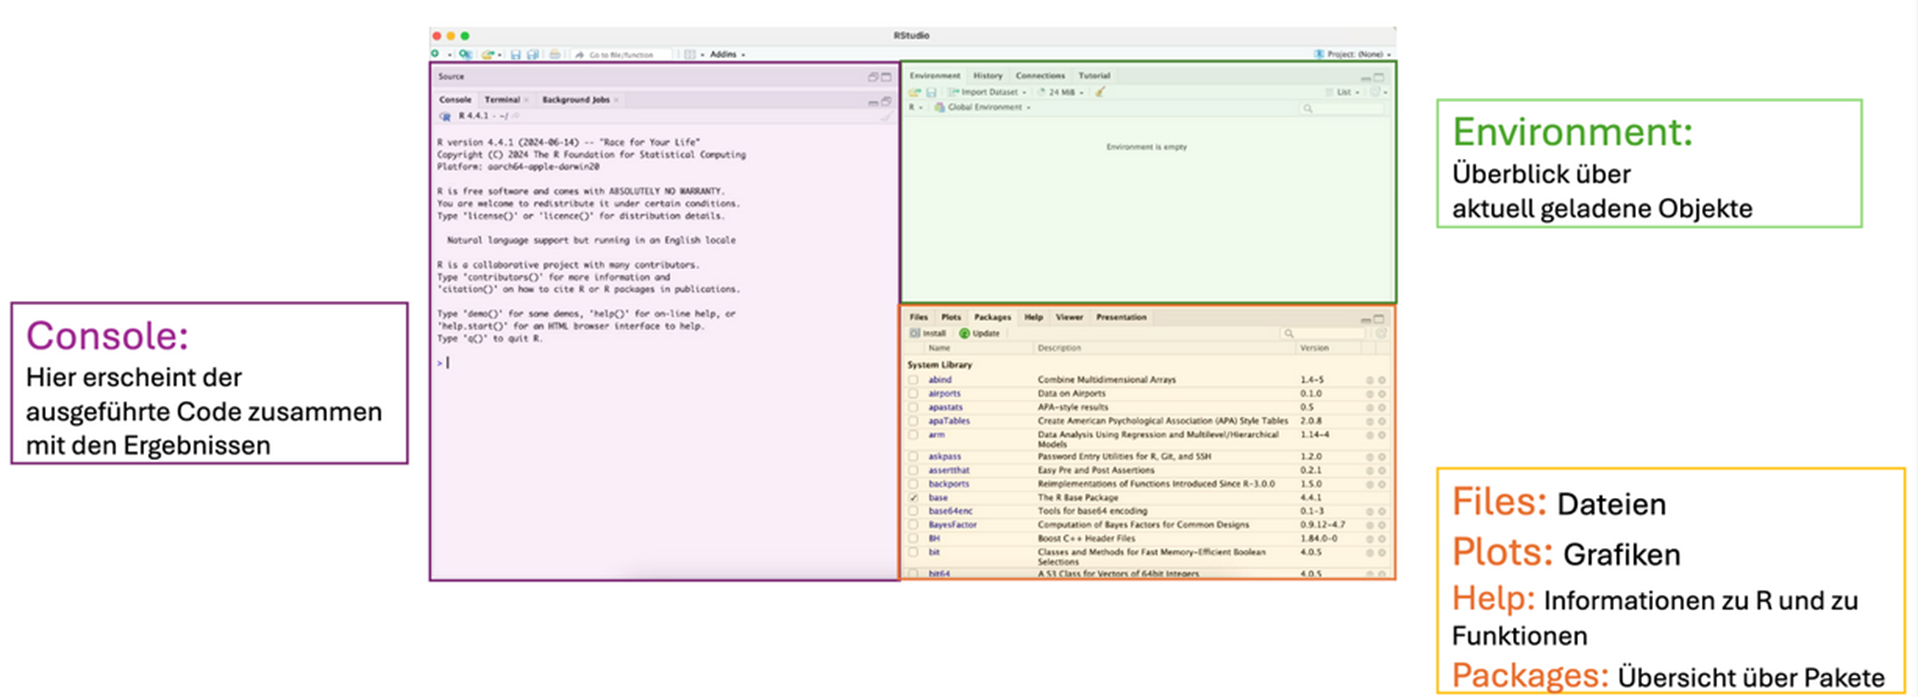
\includegraphics[keepaspectratio]{images/clipboard-2744485803.png}}

\subsection{Die
R-Studio-Arbeitsumgebung}\label{die-r-studio-arbeitsumgebung-1}

Da wir in R-Studio aber immer mit Skripten arbeiten, sieht die
Oberfläche typischerweise so aus:

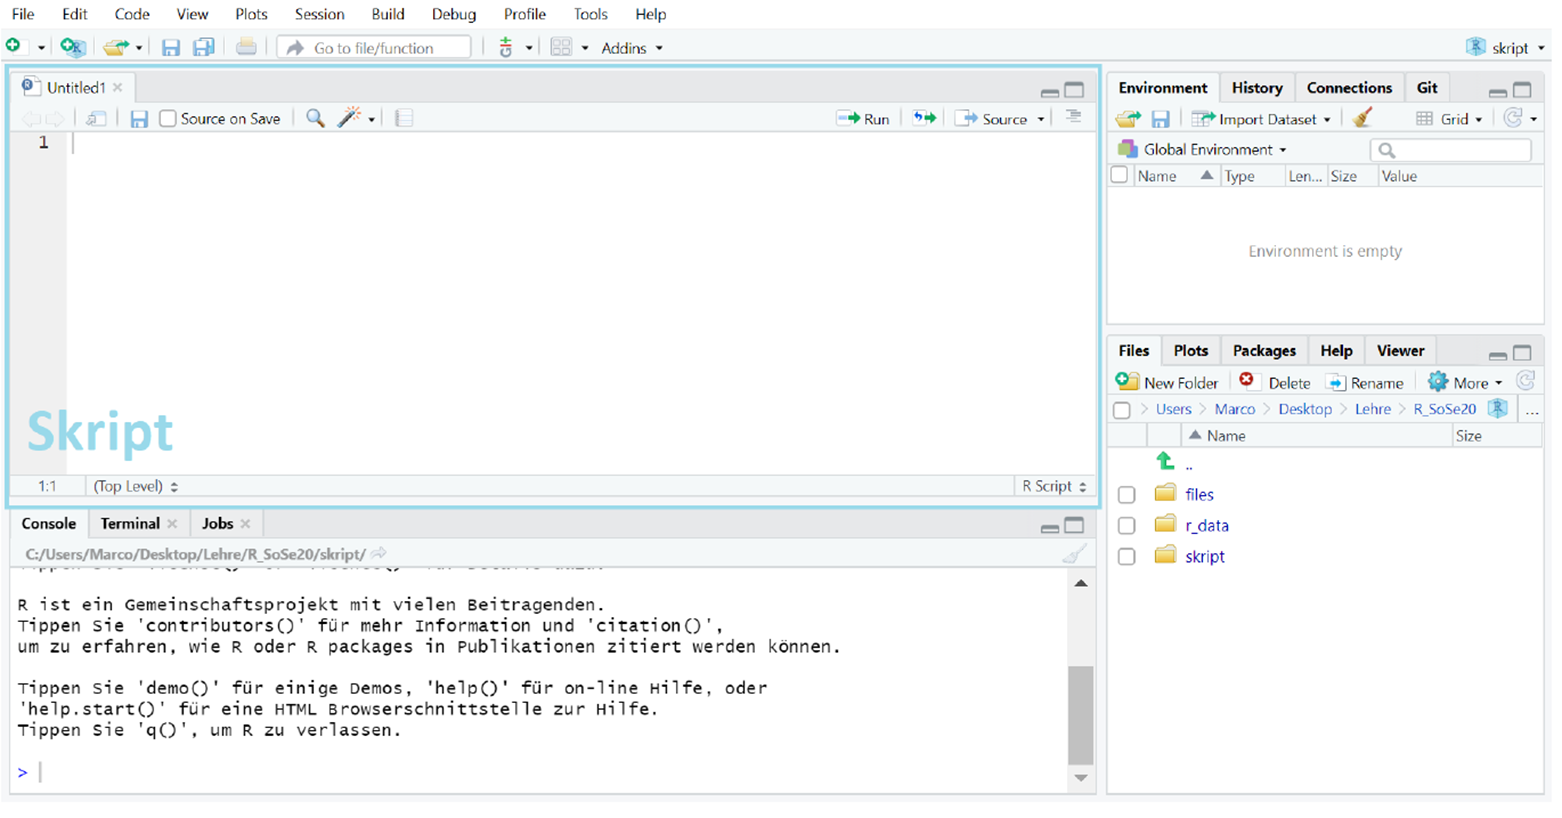
\includegraphics[width=1\linewidth,height=\textheight,keepaspectratio]{images/clipboard-3365166862.png}

\subsection{Einstellungen}\label{einstellungen}

\begin{itemize}
\tightlist
\item
  Tools → Global Options
\item
  Bitte die Optionen zum Workspace deaktivieren: Häkchen nicht setzen
  und im drop-down-Menü ``never'' wählen
\item
  mehr Infos zu den Einstellungen im
  \href{https://docs.posit.co/ide/user/}{User Guide}
\end{itemize}

\pandocbounded{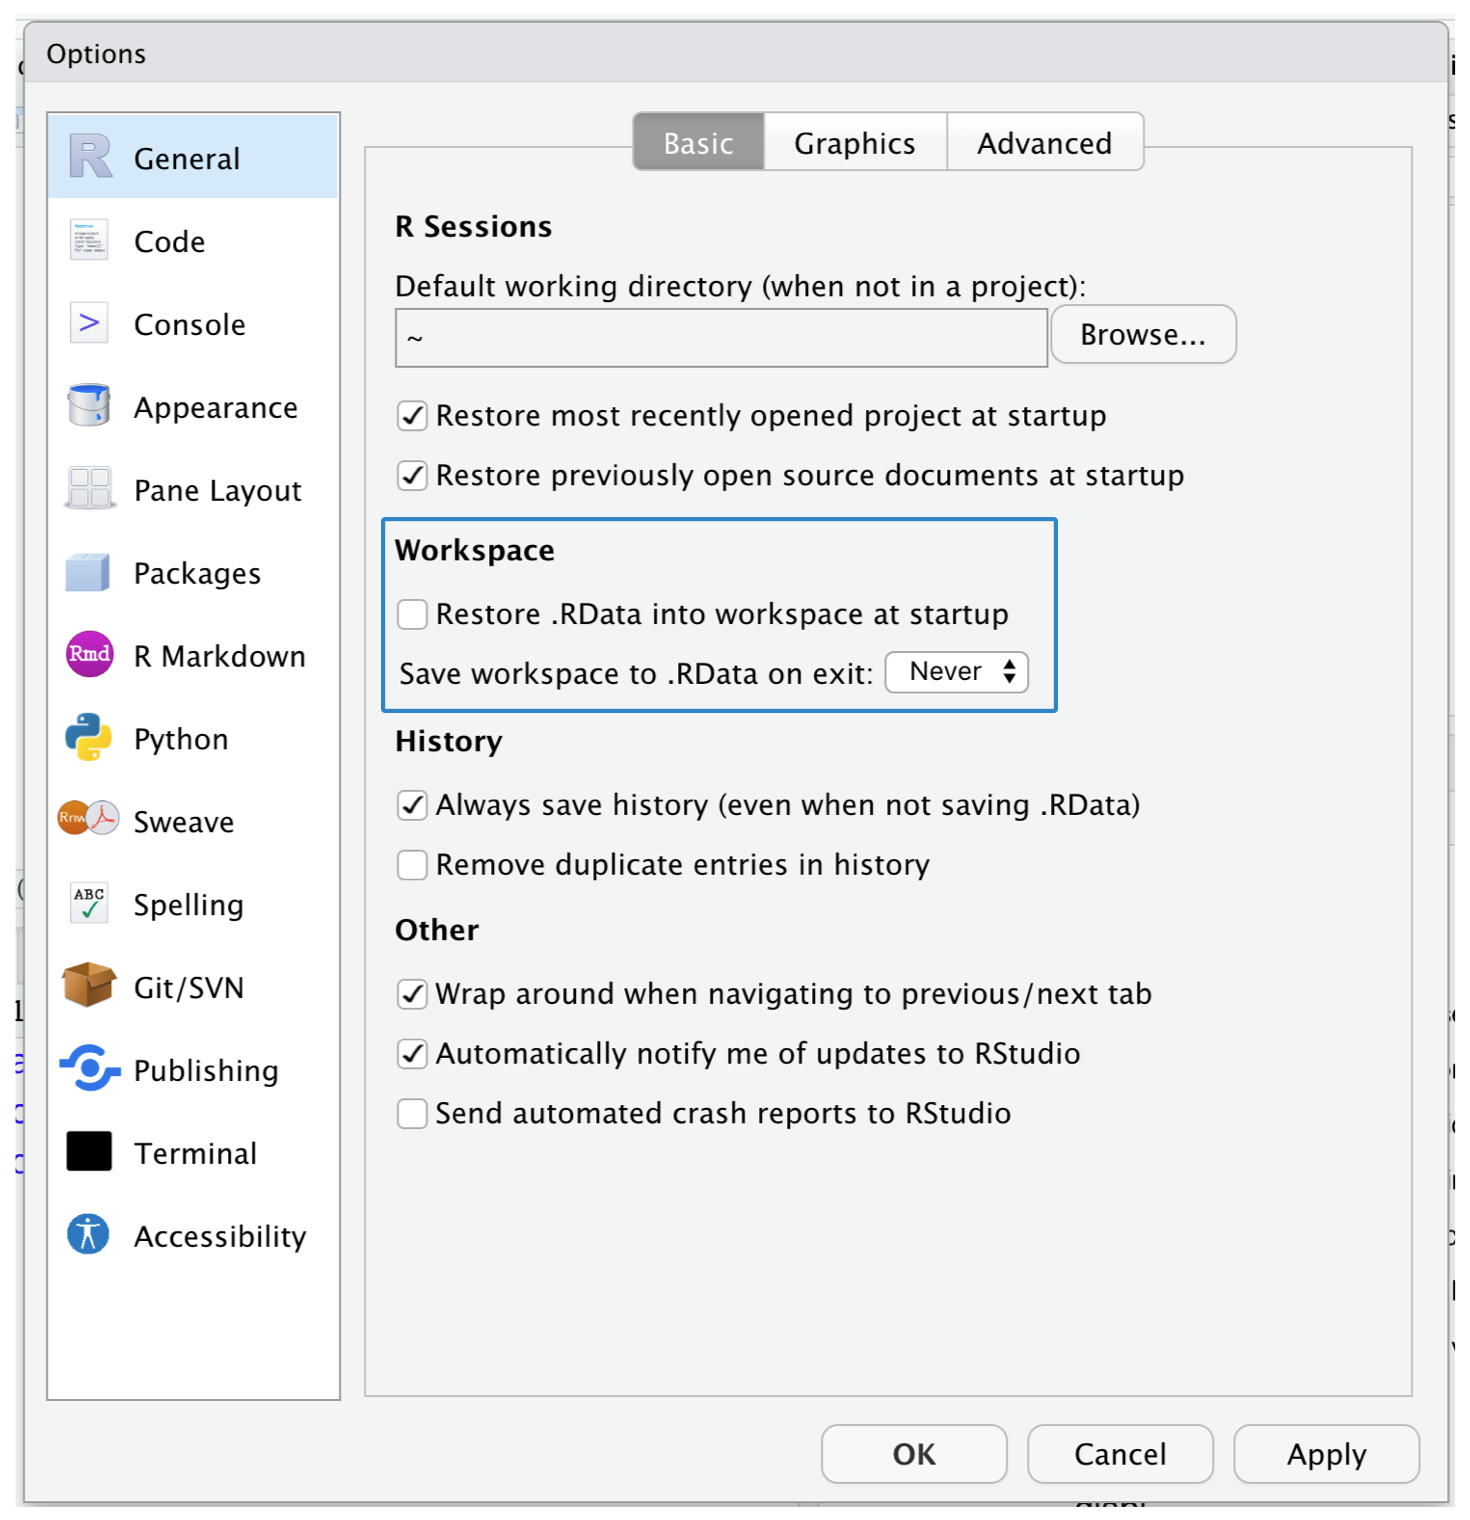
\includegraphics[keepaspectratio]{images/clipboard-3291071677.png}}

\subsection{Ordner und Pfade}\label{ordner-und-pfade}

\begin{itemize}
\tightlist
\item
  Wir müssen R sagen, wo es Datensätze einlesen und Ergebnisse ablegen
  soll
\item
  Dazu ist es sinnvoll in Projekten zu arbeiten (1 Projekt pro Kurs/
  Hausarbeit/ Forschungsprojekt)
\item
  So müssen nicht immer lange, nicht reproduzierbare absolute Pfade
  \textbf{angegeben} werden
\item
  Und es muss nicht immer explizit der Arbeitsordner mit
  \texttt{setwd("Pfad-zum-Ordner")} festgelegt werden
\item
  Ein \textbf{Projekt} legt einen Ordner als Standard-Arbeitsordner fest
\item
  Von dort aus können dann unterschiedliche Unterordner mit relativen
  Pfaden angesteuert werden:
  \texttt{haven::read\_csv("./data/dataset1.csv")}
\end{itemize}

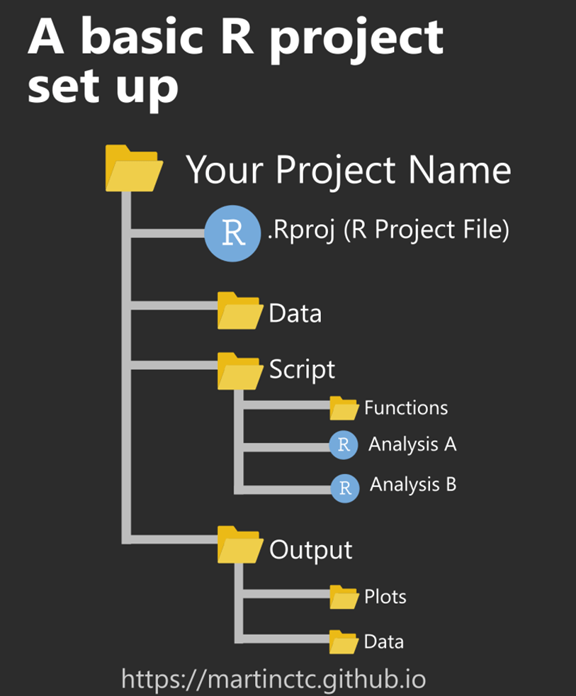
\includegraphics[width=1\linewidth,height=\textheight,keepaspectratio]{images/clipboard-1445146113.png}

\subsection{Die wichtigsten
Keyboard-Shortcuts}\label{die-wichtigsten-keyboard-shortcuts}

\begin{itemize}
\item
  Über \texttt{Strg.\ +\ Shift\ +\ F10}. starten wir die Sitzung neu.
  Alternativ können wir R-Studio schließen und erneut öffnen.
\item
  \texttt{Str\ +\ Enter} führt Code aus. Dafür:

  \begin{itemize}
  \item
    entweder den auszuführenden Code markieren
  \item
    oder den Cursor irgendwo im auszuführenden Code-Chunk platzieren
  \end{itemize}
\item
  \texttt{Str\ +\ Shift\ +\ S} führt das gesamte Skript aus.
\item
  \texttt{Str\ +\ Shift\ +\ M} fügt die Pipe
  (\texttt{\%\textgreater{}\%}) ein
\item
  \texttt{Str\ +\ Shift\ +\ L} räumt die Console auf
\end{itemize}

\subsection{Guter Stil im Skript}\label{guter-stil-im-skript}

\begin{enumerate}
\def\labelenumi{\arabic{enumi}.}
\item
  erkläre, was du tust in \texttt{\#\ Kommentaren}
\item
  benne Objekte ausschließlich mit Kleinbuchstaben und trenne Wörter mit
  \texttt{\_}

\begin{verbatim}
i_use_snake_case 
otherPeopleUseCamelCase 
some.people.use.periods 
And_aFew.People_RENOUNCEconvention
\end{verbatim}
\item
  unterteile dein Skript in Sektionen

\begin{verbatim}
# Load data --------------------------------------

# Plot data --------------------------------------
\end{verbatim}
\end{enumerate}

\begin{tcolorbox}[enhanced jigsaw, coltitle=black, toprule=.15mm, breakable, colframe=quarto-callout-note-color-frame, leftrule=.75mm, arc=.35mm, opacitybacktitle=0.6, title=\textcolor{quarto-callout-note-color}{\faInfo}\hspace{0.5em}{Note}, rightrule=.15mm, colback=white, titlerule=0mm, bottomtitle=1mm, toptitle=1mm, bottomrule=.15mm, left=2mm, opacityback=0, colbacktitle=quarto-callout-note-color!10!white]

Mehr dazu

im \href{https://style.tidyverse.org/}{Tidyverse-Styleguide} und im
eBook \href{https://r4ds.hadley.nz/workflow-style.html}{R For Data
Science}

\end{tcolorbox}

\subsection{Guter Stil im Code}\label{guter-stil-im-code}

\begin{enumerate}
\def\labelenumi{\arabic{enumi}.}
\item
  Leerzeichen vor Operatoren (außer \texttt{\^{}}), vor
  \texttt{\%\textgreater{}\%} und vor \texttt{+} in ggplot2-Befehlen
\item
  keine Leerzeichen vor oder nach Klammern
\item
  neue Argumente/ Befehle kommen in eine neue Zeile
\item
  Pipes sollten grundsätzlich das letzte in einer Codezeile sein
\item
  eine Pipe sollte nicht länger als 10-15 Zeilen sein
\end{enumerate}

\subsection{Basic R-Syntax}\label{basic-r-syntax}

\begin{itemize}
\item
  \texttt{\#} für Kommentare, also Beschreibungen
\item
  \texttt{\textless{}-} um etwas einem R-Objekt zuzuweisen
\item
  \texttt{{[}{]}} um Positionen anzugeben
\item
  Durch Drücken der Tab-Taste erhältst du Vorschläge zur
  Vervollständigung
\end{itemize}

\subsection{Funktionen}\label{funktionen}

\texttt{function\_name(argument1\ =\ value1,\ argument2\ =\ value2,\ ...)}

\subsection{Nützliche Befehle}\label{nuxfctzliche-befehle}

\begin{itemize}
\item
  \texttt{ls()} zeigt alle Objekte
\item
  \texttt{rm()} für ``remove'' löscht ein Objekt
\end{itemize}

\begin{tcolorbox}[enhanced jigsaw, coltitle=black, toprule=.15mm, breakable, colframe=quarto-callout-note-color-frame, leftrule=.75mm, arc=.35mm, opacitybacktitle=0.6, title=\textcolor{quarto-callout-note-color}{\faInfo}\hspace{0.5em}{Befehle ausführen}, rightrule=.15mm, colback=white, titlerule=0mm, bottomtitle=1mm, toptitle=1mm, bottomrule=.15mm, left=2mm, opacityback=0, colbacktitle=quarto-callout-note-color!10!white]

\texttt{Str\ +\ Enter} führt den Befehl aus. Dafür:

\begin{itemize}
\item
  entweder den auszuführenden Code markieren
\item
  oder den Cursor irgendwo im auszuführenden Code-Chunk platzieren
\end{itemize}

\end{tcolorbox}

\begin{tcolorbox}[enhanced jigsaw, coltitle=black, toprule=.15mm, breakable, colframe=quarto-callout-note-color-frame, leftrule=.75mm, arc=.35mm, opacitybacktitle=0.6, title=\textcolor{quarto-callout-note-color}{\faInfo}\hspace{0.5em}{Skript ausführen}, rightrule=.15mm, colback=white, titlerule=0mm, bottomtitle=1mm, toptitle=1mm, bottomrule=.15mm, left=2mm, opacityback=0, colbacktitle=quarto-callout-note-color!10!white]

Str + Shift + S führt das gesamte Skript aus

\end{tcolorbox}

\subsection{Wo bekomme ich Hilfe?}\label{wo-bekomme-ich-hilfe}

\begin{enumerate}
\def\labelenumi{\arabic{enumi}.}
\item
  Direkt in R-Studio

  \begin{itemize}
  \item
    \texttt{?befehl()}, z.B. \texttt{?mean()}
  \item
    \texttt{?paket}, z.B. \texttt{?dplyr}
  \item
    \texttt{??"stichwort"}, z.B. \texttt{??"mean"}
  \end{itemize}
\item
  Von Kommiliton*innen
\item
  Von mir während der Sitzung und/ oder in Sprechstunden
\end{enumerate}

\pandocbounded{
\includegraphics[keepaspectratio]{images/clipboard-2852768130.png}}

\subsection{Wo bekomme ich Hilfe ?}\label{wo-bekomme-ich-hilfe-1}

\begin{enumerate}
\def\labelenumi{\arabic{enumi}.}
\setcounter{enumi}{3}
\item
  Online

  \begin{itemize}
  \tightlist
  \item
    bei
    RStudio/\href{https://support.posit.co/hc/en-us/articles/200552336-Getting-Help-with-R}{Posit}
  \item
    über die von Google betriebene Suchmaschine
    \href{https://www.rseek.org/}{Rseek}
  \item
    auf der \href{https://cran.r-project.org/}{CRAN-Webseite} unter
    ``Manuals'' gibt es hilfreiche Einstiegshandbücher
  \item
    auf \href{https://www.datacamp.com/doc/r/r-tutorial}{Datacamp} für
    einen schnellen Überblick über Basics
  \item
    in den Ressourcen im Syllabus
  \end{itemize}
\end{enumerate}

\section{sitzung 3 ?}\label{sitzung-3}

\subsection{Überblick}\label{uxfcberblick}

\begin{itemize}
\item
  glimpse()
\item
  summary()
\item
  summarytools::dfSummary()
\end{itemize}

\subsection{Datentransformation mit
dplyr}\label{datentransformation-mit-dplyr}




\end{document}
